\documentclass{article}
\usepackage{graphicx} % Required for inserting images
\usepackage{amsmath}
\usepackage{mathalfa}
\usepackage{blindtext}
\usepackage[letterpaper, portrait, margin=0.75in]{geometry}
\usepackage{amssymb}
\usepackage{epsf, subfigure, verbatim, epsfig}
\usepackage{fancyhdr}
\usepackage{calc}
\usepackage{ifthen}
\usepackage{layout}
\usepackage{fancybox}
\usepackage{eurosym}
\usepackage{tabularx}
\usepackage{xspace}
\usepackage{dsfont,mathrsfs}
\usepackage{amssymb}
\usepackage{theorem}
\usepackage{multicol}
\usepackage{float}
\usepackage{tikz}
\usepackage{pgfplots}
\pgfplotsset{compat=1.18}

\title{Portfolio \\ \large MATH 476}
\author{Ahad Jiva}

\begin{document}

\maketitle
\section*{Exercise 1} 
\begin{flushleft}
    \textbf{Forward Contract Payoff}
    \begin{enumerate}
        \item The payoff from a long position (buying the asset) in a forward contract is $S_T - K$.
        \item The payoff from a short position (selling the asset) in a forward contract is $K - S_T$.
    \end{enumerate}
\end{flushleft}
\section*{Exercise 2}
\begin{flushleft}
    \textbf{Forward Contract on Stock Index} \\
    We know the current price is \$1000 and the 6-month forward price is \$1020.
    \begin{enumerate}
        \item If the price is \$950 in 6 months, the long position will lose \$70 (950 - 1020).
        \item If the price is \$1200 in 6 months, the long position will gain \$180 (1200 - 1020).        
    \end{enumerate}
    The forward contract allows for a profit if the value of the asset increases after 6 months, without having to actually own the asset.
    \\ Payoff Diagram:
    \begin{center}
        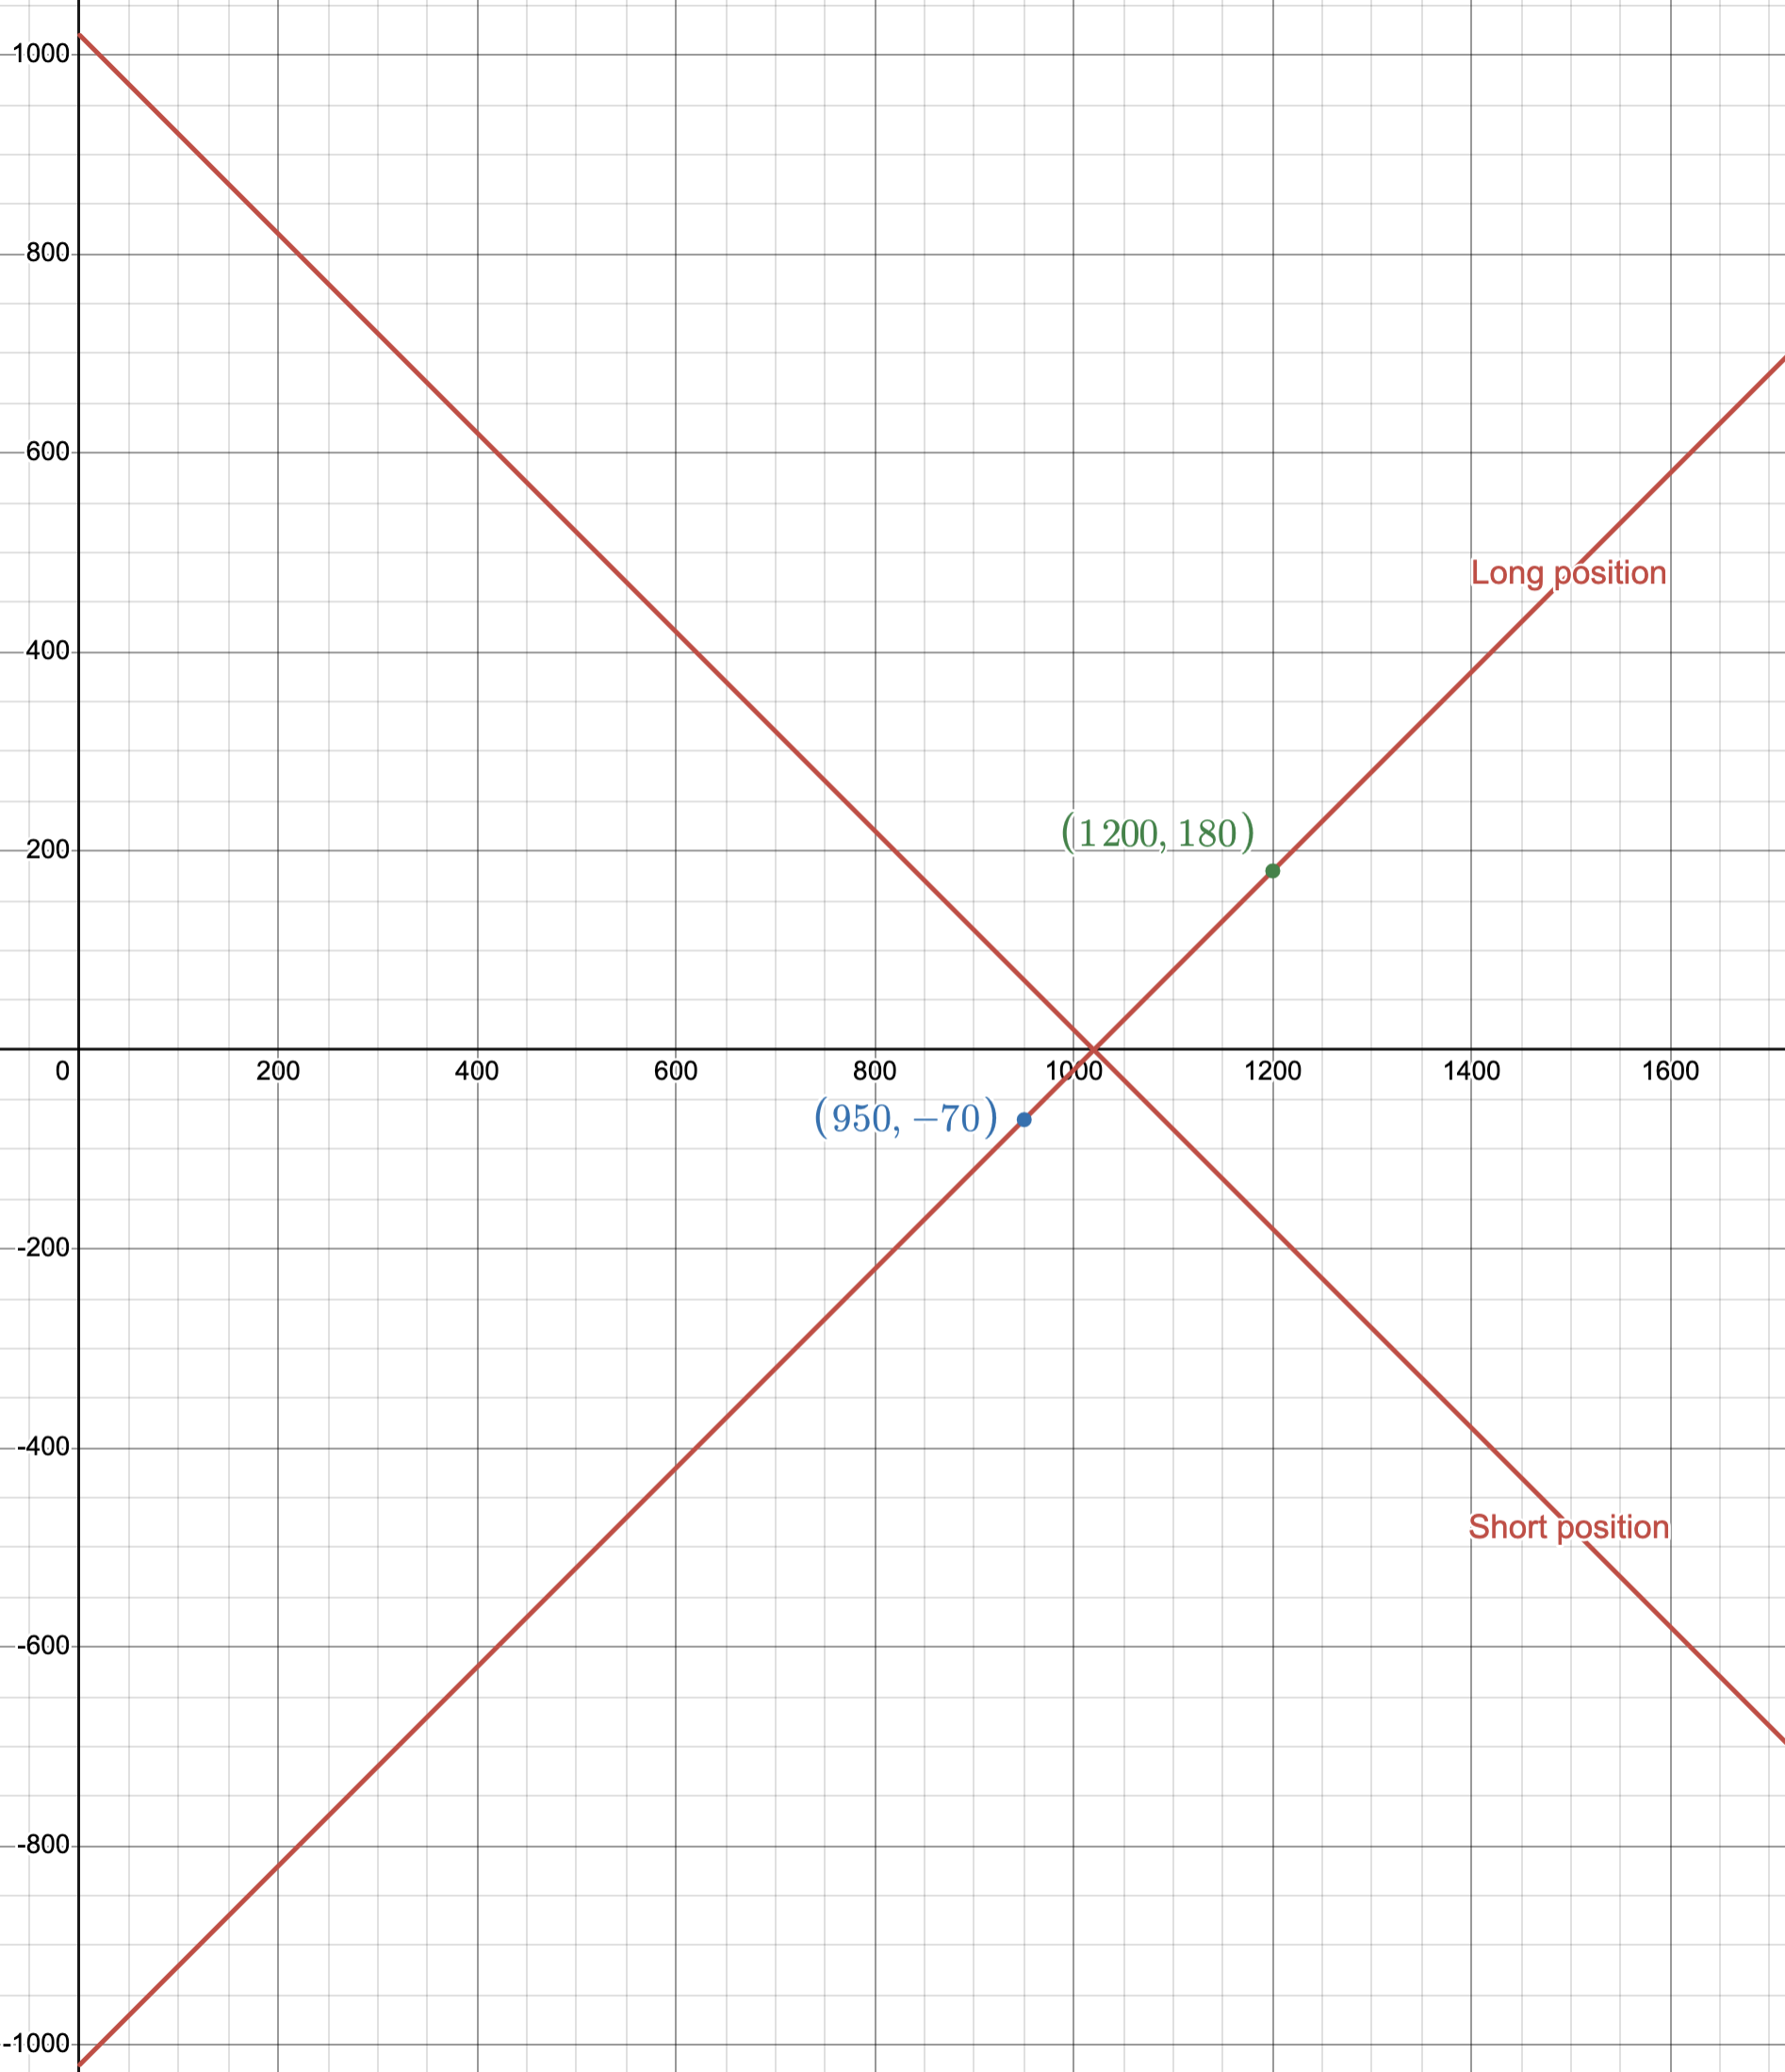
\includegraphics[width=0.5\textwidth]{figures/ex2.png}
    \end{center}
\end{flushleft}

\section*{Exercise 3}
\begin{flushleft}
    \textbf{Payoff Diagrams for Forward Contract}
\end{flushleft}
\begin{center}
    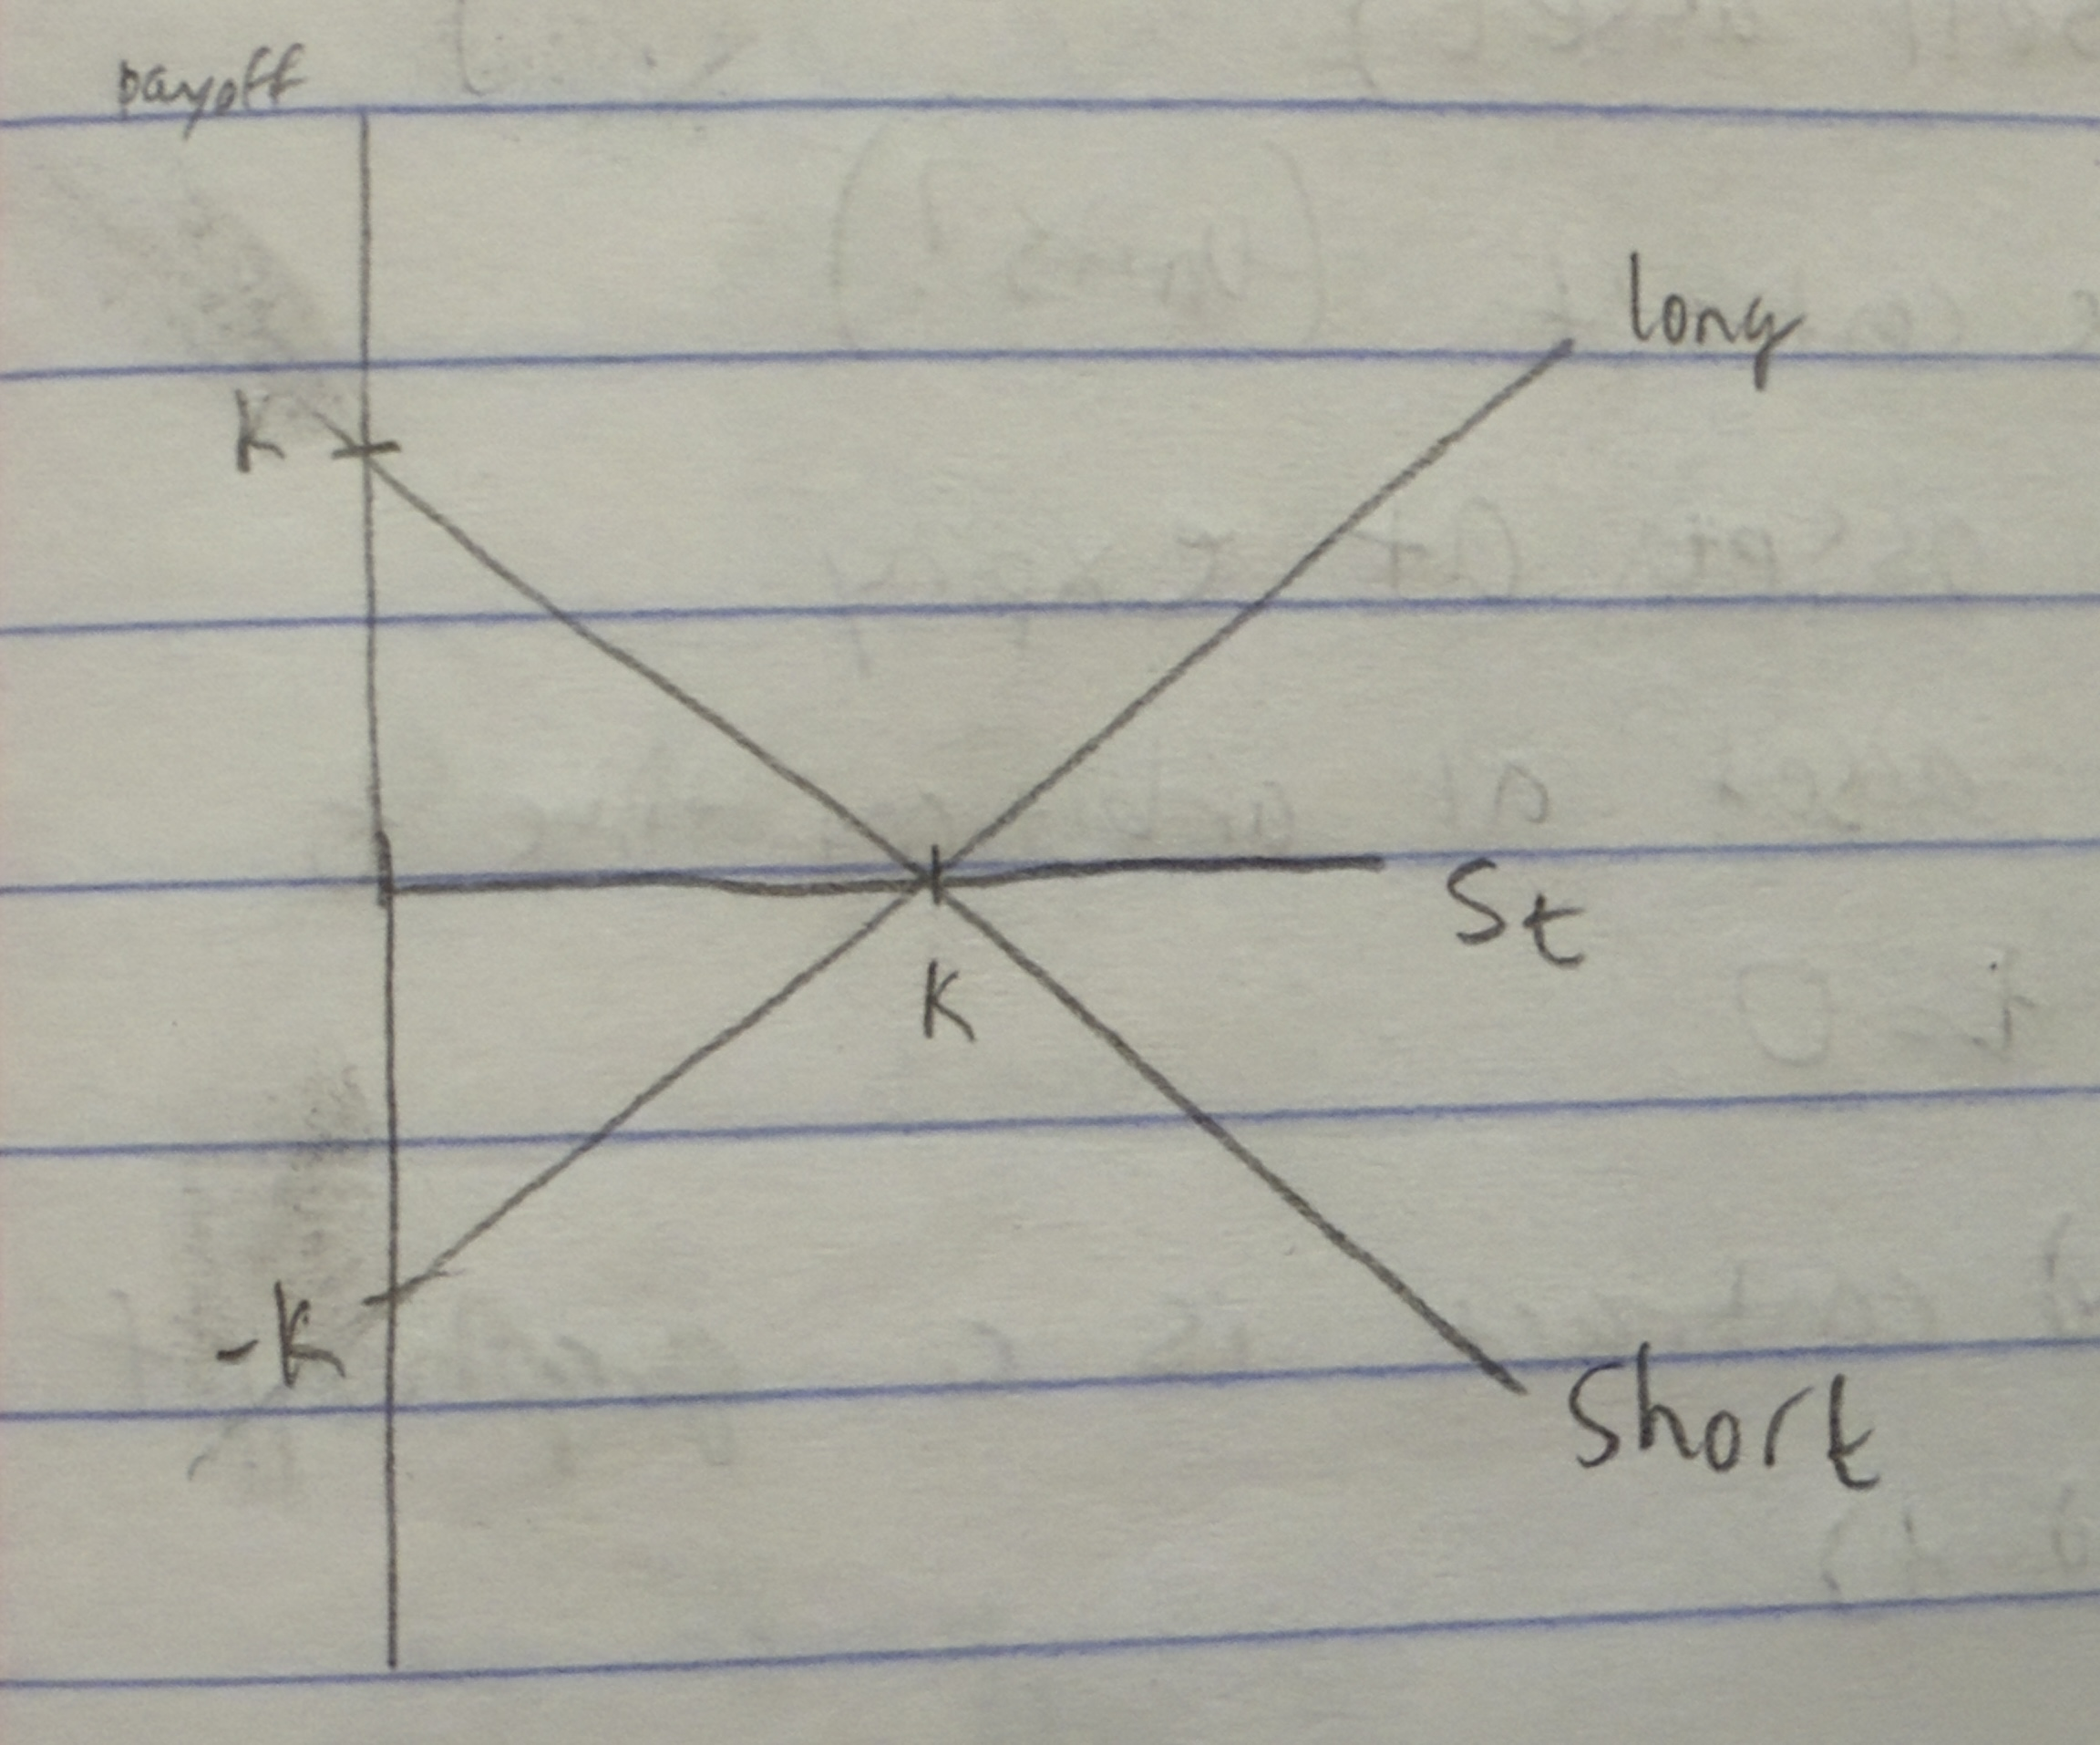
\includegraphics[width=0.5\textwidth]{figures/ex3.jpg}
\end{center}

\section*{Exercise 4}
\begin{flushleft}
    \textbf{Forward Contract on Foreign Exchange} \\
    The bank agrees to a 6-month forward contract to purchase 1 million GBP in 6 months.
    \begin{enumerate}
        \item If the spot price is 1.3000 in 6 months, the bank will make $(1.3000 - 1.2230) \cdot 1000000 = \$77000$.
        \item If the spot price is 1.2000 in 6 months, the bank will lose $(1.2000 - 1.2230) \cdot 1000000 = \$23000$.
    \end{enumerate}
\end{flushleft}

\section*{Exercise 5}
\begin{flushleft}
    \textbf{Forward Contract on Foreign Exchange} \\
    An investor enters into a short forward contract to sell 100,000 GBP for USD at 1.3000 USD per pound.
    \begin{enumerate}
        \item If the spot price is 1.2900 at the end of the contract, the short position gains $(1.3000 - 1.2900) \cdot 100000 = \$1000$.
        \item If the spot price is 1.3200 at the end of the contract, the short position loses $(1.3000 - 1.3200) \cdot 100000 = \$2000$.
    \end{enumerate}
\end{flushleft}

\section*{Exercise 6}
\begin{flushleft}
    \textbf{Forward Contract on Foreign Exchange} \\
    A trader enters into a short forward contract to sell 100 million yen at \$0.0090 per yen.
    \begin{enumerate}
        \item If the spot price is 0.0084 at the end of the contract, the short position gains $(0.0090 - 0.0084) \cdot 100000000 = \$ 60000$.
        \item If the spot price is 0.0101 at the end of the contract, the short position loses $(0.0090 - 0.0101) \cdot 100000000 = \$ 110000$.
    \end{enumerate}
\end{flushleft}

\section*{Exercise 7}
\begin{flushleft}
    ECO with T = 10 days, K = \$250
    \begin{enumerate}
        \item If $S_T = \$270$, then the holder of the ECO will exercise the option and the payoff will be $270 - 250 = \$20$
        \item If $S_T = \$230$, then the holder of the ECO will let the option expire worthless. The payoff is zero and the holder of the option only loses the option premium.        
    \end{enumerate}
\end{flushleft}

\section*{Exercise 8}
\begin{flushleft}
    Expected Value = $\frac{1}{2} \cdot \$20 + \frac{1}{2} \cdot \$0 = \$10$
\end{flushleft}

\section*{Exercise 9}
\begin{flushleft}
    Suppose that an investor did indeed pay c = 10 dollars for an ECO.
    \begin{enumerate}
        \item If $S_T = \$270$, then the payoff is \$20. The net profit is $20 - 10 = \$10$. In this case the net profit is $100\%$ of the initial cost.
        \item If $S_T = \$230$, then the payoff is \$0. The net profit is $0 - 10 = -\$10$. In this case, the loss is  $100\%$ of the initial cost.
    \end{enumerate}
\end{flushleft}

\section*{Exercise 10}
\begin{flushleft}
    Suppose that the investor purchases the stock for \$250 outright instead of buying an option.
    \begin{enumerate}
        \item If $S_T = \$270$, then the profit is \$20, which is 8\% of the initial cost.
        \item If $S_T = \$230$, then the profit is -\$20, which is also 8\% of the initial cost.
    \end{enumerate}
    Compared to buying a call option, purchasing the stock outright has less risk in terms of potential percentage gained or lost. However, the initial cost is much higher.
\end{flushleft}

\section*{Exercise 11}
\begin{flushleft}
    EPO with 100 shares of underlying stock, $K = \$70$, current price is \$65. If $S_T = \$55$, then the holder will exercise the option.
    The payoff will be $100 \cdot (70 - 55) = \$1500$.
\end{flushleft}

\section*{Exercise 12}
\begin{flushleft}
    ECO with $K = \$100$, 100 underlying shares, $c = \$500$, $S_T = \%102$.
    \begin{enumerate}
        \item Option 1: Exercise option. The per-share gain is \$2, so the total gain is \$200. Subtracting the \$500 initial cost, the investor would lose \$300.
        \item Option 2: Let option expire worthless. The total gain is \$0 and the option cost \$500, so the total loss is \$500.
    \end{enumerate}
    In this case, exercising the option would let the investor reduce their losses.
\end{flushleft}

\section*{Exercise 13}
\begin{flushleft}
    \begin{enumerate}
        \item Long position in ECO: If $S_T \leq K$, the long position lets the option expire worthless. The payoff is 0. If $S_T > K$, the long position exercises the option. The payoff is $S_T - K$.
            Thus, the payoff is $\text{max}(S_T-K, 0)$.
        \item Short position in ECO: If $S_T \leq K$, then the long will let the option expire and the payoff to the short is 0. If $S_T > K$, the long will exercise and the payoff to the short is $K - S_T$.
        Thus, the payoff is $\text{min}(K-S_T, 0)$.
        \item Long position in EPO: If $S_T \leq K$, then the payoff will be $K - S_T$. If $S_T > K$, then the payoff will be 0.
        \item Short position in EPO: If $S_T \leq K$, then the payoff is $S_T-K$. If $S_T > K$, then the payoff will be 0. So the payoff is $\text{min}(S_T-K, 0)$.
    \end{enumerate}
\end{flushleft}

\section*{Exercise 14}
\begin{center}
    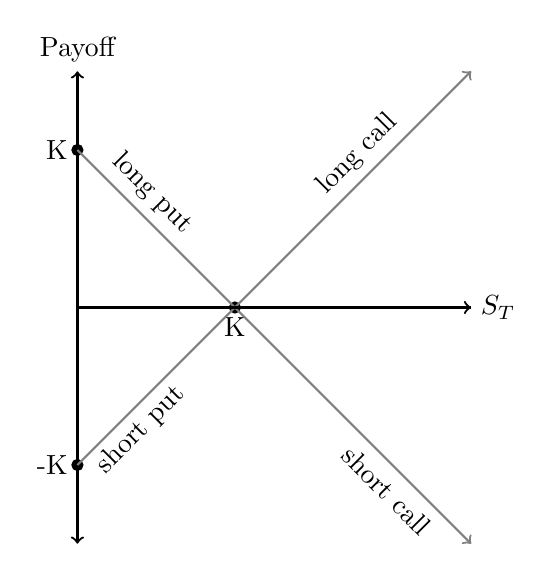
\begin{tikzpicture}
        \draw[black, thick] [<->] (-5,-1) -- (-5, 5);
        \draw[black, thick] [->] (-5,2) -- (0,2);
        \filldraw[black] (-5,4) circle (2pt) node[anchor=east]{K};
        \filldraw[black] (-3,2) circle (2pt) node[anchor=north]{K};
        \filldraw[black] (-5,0) circle (2pt) node[anchor=east]{-K};
        \draw[gray, thick] [->] (-5,4) -- (0,-1);
        \draw[gray, thick] [->] (-5,0) -- (0,5);
        \filldraw[black] (0,2) circle (0pt) node[anchor=west]{$S_T$};
        \filldraw[black] (-5,5) circle (0pt) node[anchor=south]{Payoff};
        \filldraw[black] (-4.25, 3.25) circle (0pt) node[anchor=south, rotate=-45]{long put};
        \filldraw[black] (-4, 0.25) circle (0pt) node[anchor=south, rotate=45]{short put};
        \filldraw[black] (-1.25, 3.75) circle (0pt) node[anchor=south, rotate=45]{long call};
        \filldraw[black] (-1.25, -0.5) circle (0pt) node[anchor=south, rotate=-45]{short call};
        \filldraw[black, thick] (-5, 2) -- (0,2);
    \end{tikzpicture}
\end{center}

\section*{Exercise 15}
Investor buys EPO for \$3, current price is \$42, and $K=\$40$. The profit is calculated as
    \begin{center}
        $\begin{cases}
            40 - S_T - 3 & S_T < 40 \\
            -3 & S_T \geq 40
        \end{cases}$
    \end{center}
Since we want the trade to be profitable, we want $40 - S_T - 3 > 0$, or $S_T < 37$. The option will be exercised if $S_T \leq 40$, since that means the payoff will be positive (but not necessarily the profit).
The profit diagram is as follows:
\begin{center}
    \begin{tikzpicture}
        \begin{axis}[xmin=0, xmax=49, ymin=-10, ymax=41, axis lines = middle];
        \addplot[domain=0:40]{37-x};
        \addplot[domain=40:49] [->] {-3};            
        \end{axis};
    \filldraw[black] (-0.5,6) circle (0pt) node[anchor=south]{Profit};
    \filldraw[black] (7, 1) circle (0pt) node[anchor=west]{$S_T$};
    \end{tikzpicture}
\end{center}

\break

\section*{Exercise 16}
Investor sells ECO for \$4, $K = \$50$, current price is \$47. The profit is calculated as
\begin{center}
    $\begin{cases}
        0 + 4 & S_T \leq 0 \\
        50 - S_T + 4 & S_T > 50
    \end{cases}$
\end{center}
Since we want the trade to be profitable, we want $S_T \leq 54$. The option will be exercised when $S_T < 50$, since this is when the payoff is acceptable.
The profit diagram is as follows:
\begin{center}
    \begin{tikzpicture}
        \begin{axis}[xmin=0, xmax=69, ymin=-2, ymax=5, axis lines=middle];
            \addplot[domain=0:50]{4};
            \addplot[domain=50:55] [->] {54-x};            
        \end{axis}
    \filldraw[black] (-0.5,5.75) circle (0pt) node[anchor=south]{Profit};
    \filldraw[black] (7, 1.5) circle (0pt) node[anchor=west]{$S_T$};
    \end{tikzpicture}
\end{center}

\section*{Exercise 17}
The investor has a short position on an ECO and a long position on an EPO. There are two cases to consider:
\begin{enumerate}
    \item The long position will exercise if $S_T > K$. Thus, the investor will have to sell to the long position for $K$. At time $t=T$, the payoff is
    
    $\begin{cases}
        0 & S_T \leq K \\
        K - S_T & S_T > K
    \end{cases}$

    or $-\text{max}\{S_T-K, 0\}$.

    \item The investor will exercise their long position on the EPO if $S_T < K$. At time $t=T$ the payoff is
    
    $\begin{cases}
        K-S_T & S_T < K \\
        0 & S_T \geq K
    \end{cases}$

    or $-\text{max}\{K-S_T, 0\}$.
\end{enumerate}
Then the overall payoff at expiry will be 
\begin{center}
    $-\text{max}\{S_T-K, 0\} + \text{max}\{K-S_T, 0\} = 
    \begin{cases}
        0 + K - S_T & S_T < K \\
        K - S_T + 0 & S_T \geq K
    \end{cases}
    = K - S_T$.
\end{center}
The payoff diagram looks like the following: 
\begin{center}
    \begin{tikzpicture}
        \draw[black, thick] [->] (-5,0) -- (-5, 5);
        \draw[black, thick] [->] (-5,2) -- (0,2);
        \filldraw[black] (-5,4) circle (2pt) node[anchor=east]{K};
        \filldraw[black] (-3,2) circle (2pt) node[anchor=north]{K};
        \draw[gray, thick] [->] (-5,4) -- (-2,1);
        \filldraw[black] (0,2) circle (0pt) node[anchor=west]{$S_T$};
        \filldraw[black] (-5,5) circle (0pt) node[anchor=south]{Payoff};
    \end{tikzpicture}
\end{center}

\section*{Exercise 18}
\begin{enumerate}
    \item Long Position on an ECO:
    $K = \$45$, $c = \$3$, expiry $t=T$. The profit is represented as
    \begin{center}
        $\begin{cases}
            S_T - 45 - 3 & S_T \geq 45 \\
            -3 & S_T < 45
        \end{cases}$
    \end{center}
    
    \item Long Position on an EPO:
    $K = \$40$, $c = \$4$, expiry $t=T$. The profit is represented as
    \begin{center}
        $\begin{cases}
            40-4-S_T & S_T < 40 \\
            -4 & S_T \geq 40
        \end{cases}$
    \end{center}
\end{enumerate}
Then the net profit is 
\begin{center}
    $\begin{cases}
        36-S_T-3 & S_T < 40 \\
        -3-4 & 40 \leq S_T \leq 45 \\
        S_T - 48 - 4 & S_T > 45
    \end{cases}$
\end{center}
The profit diagram is as follows:
\begin{center}
    \begin{tikzpicture}
        \begin{axis}[xmin=0, xmax=55, ymin=-10, ymax=35, axis lines=middle];
            \addplot[domain=0:40]{33-x};
            \addplot[domain=40:45]{-7};
            \addplot[domain=45:55] [->] {x-52};
        \end{axis};
        \filldraw[black] (7,1) circle (0pt) node[anchor=west]{$S_T$};
        \filldraw[black] (0,6) circle (0pt) node[anchor=east]{Profit};
    \end{tikzpicture}
\end{center}

\section*{Exercise 19}
An American option will always be worth as much as a European option on the same asset with the same strike price
and exercise date because if the holder of the American option doesn't exercise until the
expiry date, the option is no different from a European option. Having the right to 
exercise the option before the expiry date is an additional right that the American 
option has, and as such it must be at least as valuable as a similar European option.

\section*{Exercise 20}
\begin{tabular}{|l|l|l|l|l|}\hline
    {\em Variable} & {\em European call} & {\em European put} & {\em American call} &
    {\em American put}\\\hline
    Current stock price & + & – & + & – \\\hline
    Strike price & – & + & – & + \\\hline
    Time to expiration & ?&?&+&+\\\hline
    Volatility &+&+&+&+\\\hline
    Risk-free interest rate &+&–&+&–\\\hline
\end{tabular}

\section*{Exercise 21}

The trader will make a profit when the long position in the contract exercises, and the profit will be
$S_T - K - c$, which in this case is $S_T - 34$. So the investor will make a profit as long as $S_T \geq 34$.

\section*{Exercise 22}
The holder of the option will make a profit if the price of the stock at maturity is greater than or equal to
\$52.5. The option will be exercised if the price at maturity is greater than or equal to \$50, which means that
the condition for exercising does not necessarily result in a profit.

\begin{center}
    \begin{tikzpicture}
        \begin{axis}[xmin=40, xmax=55, ymin=-4, ymax=6.5, axis lines=middle];
            \addplot[domain=0:50]{-2.5};
            \addplot[domain=50:55] [->] {x-52.5};
        \end{axis};
        \filldraw[black] (0,6.25) circle (0pt) node[anchor=east]{Profit};
        \filldraw[black] (7.1, 2) circle (0pt) node[anchor=north]{$S_T$};
    \end{tikzpicture}
\end{center}

\section*{Exercise 23}
$K = 20$, $S_0 = 18$, $c = 2$. Suppose that $S_T = 25$. If the option is held until
September, at which the stock price is \$25, then the long position in the call
will exercise the option. Then the investor will have to buy a share for \$25 and
sell it to the long position for \$20, taking a loss of \$5. Since the trader
wrote the option and sold it for \$2, then the total cash flow is a loss of \$3.

\section*{Exercise 24}
\begin{enumerate}
    \item Trader A: forward contract, $K = 1000$, so profit is $S_T - 1000$.
    \item Trader B: call option, $c = 100$, $K = 1000$, so profit is
    \begin{center}
        $\begin{cases}
            -100 & S_T \leq K \\
            S_T - 1100 & S_T > K
        \end{cases}$
    \end{center}
\end{enumerate}
\begin{flushleft}
    So if $S_T > K$, then Trader A does better, and if $S_T \leq K$, then Trader A loses less money until $S_T = 900$, below which Trader A will lose more money than Trader B.
\end{flushleft}

\section*{Exercise 25}
\begin{enumerate}
    \item Purchasing shares outright: $S_0 = 316.50$, so upfront cost is \$31,650. If $S_T = 400$, then the per share profit is
    \$83.50, so the total profit is \$8,350. If $S_T = 300$, then the per share loss is \$16.50, so the total loss is \$1,650.
    \item Purchasing call options: $c = 21.70$, so the upfront cost is \$2,170. 
    If $S_T = 400$, then the profit is $-2170 + (400 - 320) \cdot 100 = 5,830$.
    If $S_T = 300$, we can let the options expire worthless. So the loss is \$2,170.
\end{enumerate}

\section*{Exercise 26}
On May 21, 2020, an investor owns 100 Apple shares. The investor is comparing two alternatives to limit risk. The first involves buying one December put option contract
with a strike price of \$290. The second involves instructing a broker to sell the 100 shares as soon as Apple’s
price reaches \$290. Discuss the advantages and disadvantages of the two strategies.

\textbf{Solution:} Let's look at the two possible choices separately:
\begin{enumerate}
    \item Buying a put option: $K = \$290, c = \$21.30$. Then the profit is
    \begin{center}
        $\begin{cases}
        -(21.30)(1000) & S_T > K \\
        K - S_T - 2130 & S_T \leq K
        \end{cases}$
    \end{center}
    \item Use a stop-loss to sell AAPL at \$290. This option is less risky, but it could lose out on profits if the market is volatile.
\end{enumerate}
Using a stop-loss is a less risky and simpler strategy that will ensure an investor will receive an exact amount for their shares. On the other hand,
using a put option could allow the investor to make a profit in the future if the stock price is predicted to decline. Given that the investor holds shares
at this instant, using a put option allows them to spend a portion of the value of the shares as "insurance", bounding the maximum possible loss. Also, if the market
is volatile, the stop-loss could be triggered before a breakout rally, causing the investor to lose out on potential profits.


\section*{Exercise 27}
Find the payoff from a bull spread.
\begin{enumerate}
    \item Case 1: $S_T > K_2$. Then the payoff is $(S_T - K_1) + (K_2 - S_T) = K_2 - K_1$.
    \item Case 2: $K_2 > S_T > K_1$. Then the payoff is $(0 + S_T - K_1) = S_T - K_1$.
    \item Case 3: $S_T < K_1$. Then the payoff is zero.
\end{enumerate}
So a trader that uses a bull spread is hoping that the stock price will increase.

\section*{Exercise 28} 
An investor buys for \$3 a 3-month European call with a strike price of \$30 and sells for \$1 a 3-month
European call with a strike price of \$35. Find the profit from this bull spread in each of the following cases:
\begin{enumerate}
    \item $S_T = \$25$. We know that $K_1 = \$30$ since it is the long position and that $K_2 = \$35$ since it is the short position.
    Then $S_T < K_1 < K_2$. Using the payoff form a bull spread from exercise 27, we know the payoff is 0. Then the profit is $-\$2$.
    \item $S_T = \$34$. Then $K_1 < S_T < K_2$. So we know that the payoff is $S_T - K_1$. So the payoff is \$4. Then the profit is \$2.
    \item $S_T = \$40$. Then $S_T > K_2$. So the payoff is $K_2 - K_1$, or \$5. Then the profit is \$3. 
\end{enumerate}

\section*{Exercise 29}
Find the payoff from a bear spread.
\begin{enumerate}
    \item Case 1: $S_T < K_2 < K_1$. Then the payoff is $(K_1 - S_T) + (S_T - K_2) = K_1 - K_2$.
    \item Case 2: $K_2 < S_T < K_1$. Then the payoff is $K_1 - S_T$.
    \item Case 3: $S_T > K_1$. Then the payoff is zero.
\end{enumerate}
So a trader using a bear spread is hoping that the stock price will decrease.

\section*{Exercise 30}
Long EPO, $K_1 = 35$, $c=3$. Short EPO, $K_2 =30$, $c=1$
\begin{enumerate}
    \item $S_T = 25$. Then the payoff is $K_1 - K_2 = 35-30 = 5$. The profit is $5 - 3 + 1 = \$3$.
    \item $S_T = 34$. Then the payoff is $K_1 - S_T = 35-34 = 1$. The profit is $1 - 2 = -\$1$.
    \item $S_T = 40$. Then the payoff is 0, and the profit is -\$2.
\end{enumerate}

\section*{Exercise 31}
\begin{flushleft}
Find the payoff from a straddle (long on an ECO and long on an EPO, both same strike price and expiry).
We know the payoff from the long ECO is 
\begin{center}
    $\begin{cases}
        S_T - K & S_T > K \\
        0 & S_T \leq K
    \end{cases}$
\end{center}
and the payoff from the long EPO is
\begin{center}
    $\begin{cases}
        K-S_T & S_T < K \\
        0 & S_T \geq K
    \end{cases}$
\end{center}
Then the total payoff is
\begin{center}
    $\begin{cases}
        S_T - K & S_T > K \\
        K - S_T & S_T \leq K
    \end{cases}$
\end{center}
This can be represented with the following payoff diagram
\begin{center}
    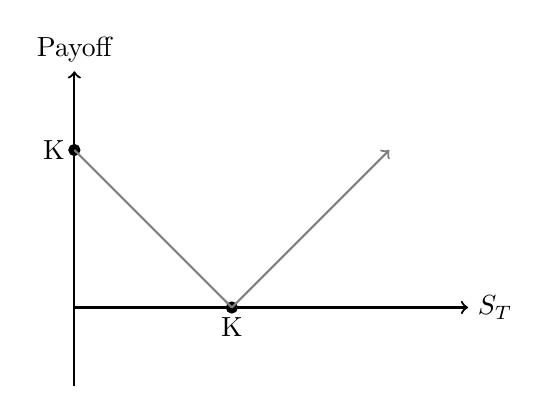
\begin{tikzpicture}
        \draw[black, thick] [->] (-5,1) -- (-5, 5);
        \draw[black, thick] [->] (-5,2) -- (0,2);
        \filldraw[black] (-5,4) circle (2pt) node[anchor=east]{K};
        \filldraw[black] (-3,2) circle (2pt) node[anchor=north]{K};
        \draw[gray, thick] (-5,4) -- (-3,2);
        \draw[gray, thick] [->] (-3,2) -- (-1,4);
        \filldraw[black] (0,2) circle (0pt) node[anchor=west]{$S_T$};
        \filldraw[black] (-5,5) circle (0pt) node[anchor=south]{Payoff};
    \end{tikzpicture}
\end{center}
\end{flushleft}

\section*{Exercise 32}
Long ECO with $K= 60$, $c=6$, and long EPO with $K = 60$, $c = 4$
\begin{enumerate}
    \item The profit from the ECO is 
        $\begin{cases}
            -6 & S_T \leq 60 \\
            S_T - 66 & S_T > 60
        \end{cases}$
    \item The profit from the EPO is
        $\begin{cases}
            56 - S_T & S_T \leq 60 \\
            -4 & S_T > 60
        \end{cases}$
\end{enumerate}
Then the total profit is
\begin{center}
    $\begin{cases}
        50 - S_T & S_T \leq 60 \\
        S_T - 70 & S_T > 60
    \end{cases}$
\end{center}
Thus there will be a loss when $50 < S_T < 70$.

\section*{Exercise 33}
Initial = 150, $r = 0.08$, find value after 20 days (365 days in a year). We use the usual formula:
$V(t) = (1 + tr)P$. Plugging in the given numbers, we get \$150.66.

\section*{Exercise 34}
We need \$1000 after 3 months with annual interest at 8\%. Using the usual formula:
$V(t) = (1 + tr)P$. We plug in the given values and isolate P to get \$980.39 of initial capital.

\section*{Exercise 35}
Initial deposit of \$100, annual interest of 10\%, find value after two years when compounded
\begin{enumerate}
    \item Annually: Then we have $V(2) = (1 + \frac{10}{1})^{2\cdot1} \cdot 100 = \$121$
    \item Monthly: Then we have $V(2) = (1 + \frac{10}{12})^{2\cdot12} \cdot 100 = \$122.03$
\end{enumerate}

\section*{Exercise 36}
Show if $m < k$, then
\begin{center}
    $(1 + \frac{r}{m})^m < (1 + \frac{r}{k})^k$
\end{center}
\begin{flushleft}
    Proof: Let $f(x) = (1 + \frac{r}{x})^x$ for $x > 0$. It is enough to show that $f(x)$ is increasing. Take the natural log of both sides and use log rules to get:
    \begin{center}
        $\ln(f(x)) = \ln((1 + \frac{r}{x})^x) = x\ln(1 + \frac{r}{x})$
    \end{center}
    Now take the derivative of both sides and simplify:
    \begin{center}
        $\frac{1}{f(x)} f'(x) = \ln(1 + \frac{r}{x}) + x(\frac{1}{1+\frac{r}{x}})(-\frac{r}{x^2})$ \\
        $f'(x) = f(x) \big(\ln(1 + \frac{r}{x}) - \frac{r}{x+r}\big)$
    \end{center}
    Observe that $f(x) > 0$, so we just need to show that the other term is positive.
    \begin{center}
        $\ln(1 + \frac{r}{x}) - \frac{r}{x+r} > 0$ \\
        $(x + r) \cdot \ln(1 + \frac{r}{x}) > r$ \\
        $e^{x+r} + (1 + \frac{r}{x}) > e^{x+r}$
    \end{center}
    We know this must be true, therefore $f'(x)$ is indeed greater than zero. So $f(x)$ is indeed increasing and we are done. $\square$
\end{flushleft}

\section*{Exercise 37}
Solve $\frac{dV}{dt} = r \cdot V$
\begin{flushleft}
    We can use separation of variables to solve this differential equation.
    \begin{center}
        $\frac{dV}{V} = r \cdot dt$
    \end{center}
    Integrate both sides:
    \begin{center}
        $\int \frac{dV}{V} = \int r \cdot dt$ \\
        $\ln(|v|) = rt + C$ \\
        $V = e^{rt + C} = Ce^{rt}$
    \end{center}
    Now we can use our initial condition to find a specific solution.
    \begin{center}
        $V(0) = 0$ \\
        $V(0) = Ce^0$ \\
        $P = C$
    \end{center}
    Thus $V = Pe^{rt}$.
\end{flushleft}

\section*{Exercise 38}
Continous compounding is given by $V(t)=\lim_{m\rightarrow\infty}\left(1+\frac{r}{m}\right)^{tm}P.$
\begin{enumerate}
    \item Show that $e=\lim_{x\rightarrow\infty}\left(1+\frac{1}{x}\right)^x.$ To start, we can take the natural log of both sides:
        \begin{center}
            $\ln(e) = \ln(\lim_{x\rightarrow\infty}(1 + \frac{1}{x})^x)$ \\
            $1 = \lim_{x\rightarrow\infty}(\ln(1 + \frac{1}{x})^x)$ \\
            $1 = \lim_{x\rightarrow\infty}(x\ln(1 + \frac{1}{x}))$ \\
            $1 = \lim_{x\rightarrow\infty}\left( \frac{\ln(1 + \frac{1}{x})}{\frac{1}{x}}\right)$
        \end{center}
        Now we can use L'Hopital's Rule to evaluate this limit:
        \begin{center}
            $1 = \lim_{x\rightarrow\infty}\left( \frac{\frac{1}{1 + \frac{1}{x}} (\frac{-1}{x^2})}{(\frac{-1}{x^2})} \right)$ \\
            $1 = \lim_{x\rightarrow\infty}(\frac{1}{1 + \frac{1}{x}}) = \frac{1}{1} = 1$
        \end{center}
        Thus we achieve the desired result.
    \item Now we want to obtain a closed form expression for $V(t)$. By using the proof above, we can assert that
        \begin{center}
            $e^r = \lim_{x\rightarrow\infty}(1 + \frac{r}{x})^x$
        \end{center}
        We know that $V(t)=\displaystyle \lim_{m\rightarrow\infty}\left(1+\frac{r}{m}\right)^{tm}P$. We can rewrite this as
        \begin{center}
            $\left( \lim_{m\rightarrow\infty} (1 + \frac{r}{m})^m \right)^t \cdot P = $ \\
            $e^{rt} \cdot P = Pe^{rt}$
        \end{center}
        Thus the closed form for $V(t)$ is $V(t) = Pe^{rt}$, and this matches our result from solving the differential equation.
\end{enumerate}

\section*{Exercise 39}
\begin{flushleft}
    Prove that $c \leq S_0$. Suppose not, for the sake of contradiction. Then $S_0 < c$. Consider the portfolio where we are short one ECO and long one share of stock.
    Then the initial cash flow is $c - S_0$, which is positive. Consider the two cases:
    \begin{enumerate}
        \item $S_T \leq K$. Then the long position in the ECO will not exercise. The payoff to the investor is $c$, which is positive.
        \item $S_T > K$. Then the long position will exercise the ECO. Then the payoff to the investor is $K - S_T + S_T = K$, which is positive.
    \end{enumerate}
    Thus we have an arbitrage opportunity, which is a contradition. Thus $c \leq S_0$. $\square$
\end{flushleft}

\section*{Exercise 40}
\begin{flushleft}
    Prove that $p \leq Ke^{-rT}$. Suppose not, for the sake of contradiction. Then $p > Ke^{-rT}$. Consider the portfolio where we are short one EPO and have $Ke^{-rT}$ in cash. Then the initial cash flow is positive.
    \begin{enumerate}
        \item Case 1: $S_T < K$. Then the payoff is $p - Ke^{-rT}$, which is positive.
        \item Case 2: $S_T \geq K$. Then the payoff is $(p - Ke^{-rT}) + K$, which is also positive.
    \end{enumerate}
    Thus we have an arbitrage opportunity, which is a contradiction. Thus $p \leq Ke^{-rT}$. $\square$
\end{flushleft}

\section*{Exercise 41}
\begin{flushleft}
    Prove that $c \geq S_0 - Ke^{-rT}$. Consider the following portfolios:
    \begin{enumerate}
        \item Portfolio A: one ECO and cash equal to $Ke^{-rT}$
        \item Portfolio B: one share of the underlying stock
    \end{enumerate}
    At expiry, the value of each portfolio is
    \begin{enumerate}
        \item Portfolio A: $\max{(S_T - K, 0)} + Ke^{-rT}e^{rT}$
        \item Portfolio B: $S_T$.
    \end{enumerate}
    Note that in all cases, the value of Portfolio A is greater than Portfolio B. So by the No-Arbitrage property, $V_0(A) \geq V_0(B)$.
    Then $c + Ke^{-rT} \geq S_0$, so $c \geq S_0 - Ke^{-rT}$. $\square$
\end{flushleft}

\section*{Exercise 42}
\begin{flushleft}
    Prove that $p \geq Ke^{-rT} - S_0$. Consider the portfolio where we are long one EPO, long one share, and borrow $Ke^{-rT}$ in cash. The initial cash flow is therefore positive. Suppose, for the sake of contradiction, that
    $p < Ke^{-rT} - S_0$. Then at expiry, the payoff will be $\max(K-S_T, 0) + S_T - Ke^{-rT}e^{rT}$, which can be simplified to $\max(0, S_T - K)$, which we know is postive. Thus we have a contradiction to the no arbitrage principle.
    Thus $p \geq Ke^{-rT} - S_0$. $\square$
\end{flushleft}

\section*{Exercise 43}
Find the lower bound of a 2-month EPO with $S_0 = 58$, $K = 65$, and $r = 0.05$.
We use the formula from above for a put option: $p \geq Ke^{-rT} - S_0$. Plugging in the given values, we find that the lower bound for this put is \$6.46.

\section*{Exercise 44}
Show that $c + Ke{-rT} = p + S_0$, i.e. show put-call parity.
\begin{flushleft}
    Consider the following portfolios:
    \begin{enumerate}
        \item Portfolio A: Long one ECO and cash equal to $Ke^{-rT}$
        \item Portfolio B: Long one EPO and one share of stock
    \end{enumerate}
    At expiry, the portfolios will be worth:
    \begin{enumerate}
        \item Portfolio A: $\max(S_T - K, 0) + Ke^{-rT}e^{-rT}$, which can be simplified to $\max(S_T, K)$.
        \item Portfolio B: $\max(K - S_T, 0) + S_T$, which can be simplified to $\max(S_T, K)$.
    \end{enumerate}
    Thus at expiry, both the portfolios are worth the same. By no-arbitrage, they must be worth the same at $t=0$, thus $c + Ke{-rT} = p + S_0$. $\square$
\end{flushleft}

\section*{Exercise 45}
\begin{flushleft}
    $S_0 = 19$, $c=1$, $K=20$, $r=0.04$, expiry in 3 months means $T = 1/4$.
    We can use put-call parity to calculate the price of a put option with same strike price and expiry.
    \begin{center}
        $c + Ke^{-rT} = p + S_0$ \\
        $1 + 20e^{-0.04 \cdot 0.25} = p + 19$ \\
        $p = 1 + 20e^{-0.04 * 0.25} - 19$ \\
        $p = 1.80$
    \end{center}
\end{flushleft}

\section*{Exercise 46}
\begin{flushleft}
    $S_0 = 130$, expiry in one year means $T=1$, $c = 20$, $p=5$, $K = 120$.
    We can use put-call parity to calculate the risk-free interest rate.
    \begin{center}
        $c + Ke^{-rT} = p + S_0$ \\
        $20 + 120e^{-r \cdot 1} = 5 + 130$ \\
        $e^{-r} = \frac{5+130-20}{120}$ \\
        $e^r = \frac{120}{115}$ \\
        $r = \ln(\frac{120}{115}) = 0.0426$ \\
    \end{center}
    Thus the risk-free interest rate is 4.26\%.
\end{flushleft}

\section*{Exercise 47}
\begin{flushleft}
    $S_0 = 31$, $c = 3$, $p = 2.25$, $K = 30$, $T = 0.25$, $r=0.1$.
    Note that put-call parity does not hold here:
    \begin{center}
        $c + Ke^{-rT} = p + S_0$ \\
        $3 + 30e^{-0.1 \cdot 0.25} = 2.25 + 31$ \\
        $32.26 \neq 33.25$
    \end{center}
    Thus we should be able to construct an arbitrage opportunity. Consider a portfolio where
    we buy the call option and short-sell the put option and the stock. At $t=0$, the cash flow is
    \begin{center}
        $-c + p + S_0 = \$30.25$
    \end{center}
    Thus we have positive cash flow at $t=0$. We can then invest this at the risk-free interest rate. At expiry, this will be worth \$31.02. At expiry, we have two cases.
    \begin{enumerate}
        \item $S_T \leq 30$. Then we let the ECO expire, the EPO will be exercised, and we return the stock we shorted. The payoff will be $0 - 30 = -30$,
                and since we started with \$31.02, we have \$1.02 profit.
        \item $S_T > 30$. Then we exercise the ECO, the EPO expires worthless, and we return the stock we shorted. The payoff is $-K + S_T - S_T = -30$.
                Since we started with \$31.02 we have \$1.02 profit.
    \end{enumerate}
    Thus in all cases, we make a profit with positive initial cash flow, and this was an arbitrage opportunity. $\square$
\end{flushleft}

\section*{Exercise 48}
$p = 2.50$, $S_0 = 47$, $r = 0.06$, $K=50$. What opportunities are there for an arbitrageur?
\begin{flushleft}
    We start with the put-call parity equation: $c + Ke^{-rT} = p + S_0$. Plugging in the given values, we reach $c + 50e^{\frac{-0.06}{12}} = 49.5$, which means that $c \geq 0$.
    Thus an arbitrageur should go long in $c + Ke^{-rT}$ and short in $p + S_0$. In all cases, there will be positive initial cash flow and positive profit at expiry.
\end{flushleft}

\section*{Exercise 49}
Put-call parity will not hold for American options because they can be exercised any time before the expiry date. This means that with enough volatility, we could violate the put-call parity equation without violating the no arbitrage principle.

\section*{Exercise 50}
Prove that it is never optimal to exercise an American call option early.
\begin{flushleft}
    It suffices to show that $c > C$, since we have already argued previously that $C \geq c$ (see Ex. 19). Suppose not, for the sake of contradiction. Then $C > c$ (here C is the price of an ACO, c is the price of an ECO). Conside the portfolio where we are short one ACO, long one ECO, both with same expiry and strike price.
    Then our initial cash flow is positive. Consider the following cases:
    \begin{enumerate}
        \item Case 1: ACO expires worthless. Then the ECO also expires worthless, and our payoff is zero. Our profit is positive.
        \item Case 2: ACO is exercised. Then the ECO is also exercised. So the payoff is zero, and our profit is positive.
    \end{enumerate}
    In all cases, we make a positive profit with positive initial cash flow. This is a contradiction to the no-arbitrage principle. Thus $c = C$.
\end{flushleft}

\section*{Exercise 51}
Show that it can be optimal to exercise an APO before expiry. Suppose that $S_0$ is 100, $K = 90$. Consider the scenario where the stock price drops to \$89 right after initiation.
If we exercise the APO, we get a payoff of $K - S_T$, which is \$1. We can then invest this amount in the risk-free interest rate, which if high enough, will net us more money than waiting for option expiry.

\section*{Exercise 52}
As the risk free interest rate increases and volatility decreases, exercising an APO early becomes more attractive because the higher interest rate means we can use the money from the exercised option to invest in a risk free asset and get a good return. Also, the low volatility means that there is little chance of a large price movement that would make exercising early attractive.

\section*{Exercise 53}
\begin{flushleft}
    Show that $S_0 - K \leq C - P \leq S_0 - Ke^{-rT}$. We split this into two inequalities and prove them separately.
    \begin{enumerate}
        \item Prove that $S_0 - K \leq C - P$. Suppose not, for the sake of contradiction, i.e. $S_0 - K > C - P$. Consider the portfolio where we are long one ACO, short one APO and one share of stock.
            Note that the initial cash flow is positive. If $S_T > K$, then the payoff at expiry is $Ke^{rT} - K$, which is positive. If $S_T \leq K$, then the payoff is also $Ke^{rT} - K$, which is positive. This is a contradiction to the no arbitrage principle, thus $S_0 - K \leq C - P$.
        \item Prove that $C - P \leq S_0 - Ke^{-rT}$. We know that $C = c$ and $P \geq p$, because it is never optimal to exercise an American option early. If we make this substitution, we get $c - p = S_0 - Ke^{-rT}$, which is put-call parity (we know this is true). Since $P \geq p$, we conclude that $C - P \leq S_0 - Ke^{-rT}$.
    \end{enumerate}
    Thus we have proved both inequalities. $\square$
\end{flushleft}

\section*{Exercise 54}
We have three call options with prices $c(K_1), c(K_2), c(K_3)$ with $K_1 < K_2 < K_3$.
We also have three put options with prices $p(K_1), p(K_2), p(K_3)$. All of these options have the same expiry.
\begin{enumerate}
    \item Show $c(K_1) \geq c(K_2)$. Suppose not for the sake of contradiction, ie $c(K_1) < c(K_2)$.
        Consider the portfolio where we are short in $c(K_2)$ and long in $c(K_1)$. The initial cash flow is $c(K_2) - c(K_1) > 0$, and let $CF_0$ represent this amount.
        \begin{enumerate}
            \item Case 1: $S_T < K_1 < K_2$. Then none of the call options will be exercised. The payoff is zero and the profit is $0 + CF_0 \cdot e^{rT}$, which is positive.
            \item Case 2: $K_1 < S_T < K_2$. Then the $c(K_1)$ option will be exercised, which is our long position. So the payoff is $S_T - K_1$ and the profit is $S_T - K_1 + CF_0 \cdot e^{rT}$, which is positive.
            \item Case 3: $K_1 < K_2 < S_T$. Then both options will be exercised. The payoff will be $S_T - K_1 - S_T + K_2 = K_2 - K_1$, which is positive, and thus the profit is $K_2 - K_1 + CF_0 \cdot e^{rT}$, which is positive.
        \end{enumerate}
        Thus in all cases, we have a risk free profit with no initial investment, ie an arbitrage opportunity. Contradition. Thus $c(K_1) \geq c(K_2)$. $\square$
    \item Show $p(K_2) \geq p(K_1)$. Suppose not for the sake of contradiction, ie $p(K_2) < p(K_1)$ or $p(K_1) - p(K_2) > 0$.
        Consider the portfolio where we are short in $p(K_1)$ and long in $p(K_2)$. Then the initial cash flow is $p(K_1) - p(K_2) > 0$, and let $CF_0$ represent this amount.
        \begin{enumerate}
            \item Case 1: $S_T < K_1 < K_2$. Then both put options will be exercised. The payoff is $S_T - K_1 + K_2 - S_T = K_2 - K_1$. So the profit is $K_2 - K_1 + CF_0 \cdot e^{rT}$, which is positive.
            \item Case 2: $K_1 < S_T < K_2$. Then the $p(K_2)$ option will be exercised. The payoff is $K_2 - S_T$ and the profit is $K_2 - S_T + CF_0 \cdot e^{rT}$, which is positive.
            \item Case 3: $K_1 < K_2 < S_T$. Then none of the put options will be exercised and the payoff is zero. Then the profit is $CF_0 \cdot e^{rT}$, which is positive.
        \end{enumerate}
        Thus in all cases, we have a risk free profit with no initial investment, ie an arbitrage opportunity. Contradiction. Thus $p(K_2) \geq p(K_1)$. $\square$
    \item Show $c(K_1) - c(K_2) \leq K_2 - K_1$. Suppose not for the sake of contradiction, ie $c(K_1) - c(K_2) > K_2 - K_1$.
        Consider the portfolio where we are short in $c(K_1)$ and long in $c(K_2)$, and also we hold cash equivalent to $(K_1 - K_2) \cdot e^{-rT}$. Then the initial cash flow is $c(K_1) - c(K_2) + (K_1 - K_2)\cdot e^{-rT}$, which we denote as $CF_0$, which is positive.
        \begin{enumerate}
            \item Case 1: $S_T < K_1 < K_2$. Then neither call option is exercised. The payoff is zero, and the profit is $CF_0 \cdot e^{rT}$.
            \item Case 2: $K_1 < S_T < K_2$. Then $c(K_1)$ is exercised. The payoff is $K_1 - S_T$, and thus the profit is $K_1 - S_T + CF_0 \cdot e^{rT}$, which is positive.
            \item Case 3: $K_1 < K_2 < S_T$. Then both call options are exercised. The payoff is $K_2 - K_1$, which when added to $CF_0\cdot e^{rT}$ to get profit is positive.
        \end{enumerate}
        Thus in all cases, we have a risk free profit with no initial investment, ie an arbitrage opportunity. Contradition. Then $c(K_1) - c(K_2) \leq K_2 - K_1$. $\square$
    \item Show $p(K_2) - p(K_1) \leq K_2 - K_1$. Suppose not for the sake of contradiction, ie $p(K_2) - p(K_1) > K_2 - K_1$.
        Consider the portfolio where we are short in $p(K_1)$ and long in $p(K_2)$, and also we hold cash equivalent to $(K_1 - K_2) \cdot e^{-rT}$. Then the initial cash flow is $p(K_1) - p(K_2) + (K_1 - K_2) \cdot e^{-rT}$, denoted as $CF_0$, which is positive.
        \begin{enumerate}
            \item Case 1: $S_T < K_1 < K_2$. Then both put options will be exercised. The payoff will be $K_2 - K_1$, which when added to $CF_0 \cdot e^{rT}$ to get profit, gives us a positive value.
            \item Case 2: $K_1 < S_T < K_2$. Then $p(K_2)$ is exercised. The payoff will be $K_2 - S_T$, which is positive. When added to $CF_0 \cdot e^{rT}$, we get a positive profit.
            \item Case 3: $K_1 < K_2 < S_T$. Then neither put option will be exercised. The payoff is zero and the total profit is $CF_0 \cdot e^{rT}$ which is positive.
        \end{enumerate}
        Thus in all cases we get a risk free profit will no initial investment, ie an arbitrage opportunity. Contradiction. Then $p(K_2) - p(K_1) \leq K_2 - K_1$. $\square$
\end{enumerate}

\section*{Exercise 55}
Convexity: $c(K_1), c(K_2), c(K_3)$ ECO prices, $K_1 < K_2 < K_3$.
\begin{enumerate}
    \item Show that $K_2 = \lambda K_1 + (1 - \lambda) K_3$, ie $\exists \lambda \in \mathbb{R}$ such that $0 < \lambda < 1$. We can use algebra to obtain $\lambda = \frac{K_3 - K_2}{K_3 - K_1}$
        Since we know $K_3 \neq K_1$ and $K_3 \neq K_2$, we know $\lambda$ is not zero and we don't have to worry about zero denominators. Since $K_1 < K_2$, $K_3 - K_1 > K_3 - K_2$. Then $\lambda < 1$. Thus $0 < \lambda < 1$ as desired. $\square$
    \item Show with $\lambda$ from part a that $c(K_2) \leq \lambda c(K_1) + (1-\lambda)c(K_3)$. Suppose not, for the sake of contradiction. Then $c(K_2) > \lambda c(K_1) + (1-\lambda)c(K_3)$.
        Consider the portfolio where we short-sell $c(K_2)$, long in $\lambda c(K_1) + (1-\lambda)c(K_3)$. The initial cash flow is $c(K_2) - \lambda c(K_1) - (1 - \lambda)c(K_3) > 0$, and we denote this value as $CF_0$.
        \begin{enumerate}
            \item Case 1: $S_T \leq K_1 < K_2 < K_3$. None of the options are exercised. Then the profit is $0 + CF_0e^{rT}$, which is positive.
            \item Case 2: $K_1 < S_T < K_2 < K_3$. Then $\lambda c(K_1)$ is exercised. The profit is $\lambda (S_T - K_1) + CF_0e^{rT}$, which is positive.
            \item Case 3: $K_1 < K_2 < S_T < K_3$. Then $\lambda c(K_1)$ and $c(K_2)$ are exercised. The profit is $K_2 - \lambda K_1 - (1 - \lambda)S_T + CF_0e^{rT}$, which is positive.
            \item Case 4: $K_1 < K_2 < K_3 < S_T$. Then all options are exercised. The profit is $0 + CF_0e^{rT}$, which is positive.
        \end{enumerate}
        Thus in all cases we get a positive profit from a positive initial cash flow, contradicting the no arbitrage principle. Thus $c(K_2) \leq \lambda c(K_1) + (1-\lambda)c(K_3)$. $\square$
\end{enumerate}

\section*{Exercise 56}
$c(K_1), c(K_2), c(K_3)$ ECO prices, $K_1 < K_2 < K_3$. Also, $K_3 - K_2 = K_2 - K_1$. All options have the same maturity. Show that $c(K_2) \leq \frac{c(K_1) + c(K_3)}{2}$.
\begin{flushleft}
    Consider the portfolio where we are long in $c(K_1), c(K_3)$ and short in 2 contracts of $c(K_2)$. The initial cash flow is $-c(K_1) - c(K_3) + 2c(K_2)$, which is positive. We will denote this value as $CF_0$.
    \begin{enumerate}
        \item Case 1: $S_T < K_1 < K_2 < K_3$. None of the call options will be exercised. The payoff is zero and the profit is $CF_0e^{rT}$, which is positive.
        \item Case 2: $K_1 < S_T < K_2 < K_3$. Then $c(K_1)$ will be exercised. The profit will be $S_T - K_1 + CF_0e^{rT}$, which is positive.
        \item Case 3: $K_1 < K_2 < S_T < K_3$. Then $c(K_1)$ and $c(K_2)$ will be exercised. The profit will be $(K_2 - K_1) - (S_T - K_2) + CF_0e^{rT}$, which is positive.
        \item Case 4: $K_1 < K_2 < K_3 < S_T$. Then all options will be exercised and the profit will be $0 + CF_0e^{rT}$, which is positive.
    \end{enumerate}
    Thus in all cases we get positive profit with a positive initial cash flow, which means the no arbitrage principle is violated. Thus $c(K_2) \leq \frac{c(K_1) + c(K_3)}{2}$ as desired. $\square$
\end{flushleft}

\section*{Exercise 57}
Same as Ex. 56 but for put options, ie show that $p(K_2) \leq \frac{p(K_1) + p(K_3)}{2}$. Consider the portfolio where we are long in $p(K_1), p(K_3)$ and short in 2 contracts of $p(K_2)$. The initial cash flow is $-p(K_1)-p(K_3) + 2p(K_2)$, which is positive. We will denote this value as $CF_0$.
\begin{enumerate}
    \item Case 1: $S_T < K_1 < K_2 < K_3$. Then all of the options will be exercised. The payoff will be zero and the profit is $0 + CF_0e^{rT}$.
    \item Case 2: $K_1 < S_T < K_2 < K_3$. Then $p(K_2)$ and $p(K_3)$ will be exercised. The profit will be $(K_3 - S_T) + (K_2 - K_1) + CF_0e^{rT}$, which is positive.
    \item Case 3: $K_1 < K_2 < S_T < K_3$. Then $p(K_3)$ will be exercised. The profit will be $(K_3 - S_T) + CF_0e^{rT}$, which is positive.
    \item Case 4: $K_1 < K_2 < K_3 < S_T$. Then none of the put options will be exercised. The payoff is zero and the profit is $0 + CF_0e^{rT}$.
\end{enumerate}
Thus in all cases we have positive profit from a positive initial cash flow, which contradicts the no-arbitrage principle. Thus $p(K_2) \leq \frac{p(K_1) + p(K_3)}{2}$ as desired. $\square$

\end{document}
